\chapter{Experimentation}
\thispagestyle{empty}
In this chapter we will discuss about our dataset preparation process. We will learn about different evaluation measures. Finally by using this evaluation matrices we will evaluate the result of our system.

\section{Dataset}
Behind the success of any machine learning algorithm dataset is the key. Unfortunately, when we start this project there were no dataset available which can be used in our system. It was a very challenging task for us to build a corpus which contains a large amount of suspicious text. It took us approximately  six month to a build a well furnished  suspicious text corpus containing 4000 suspicious text. We collect non suspicious data from a pre-build corpus[16], thanks to them. At the time of collecting data we were very careful because as a machine leaning model our system learn form what we give to it. If we give wrong data then final output we will not be accurate. \par \vspace{0.5cm}\noindent 
We mark a text as suspicious if it satisfies any one of the following criteria.

\begin{itemize}
    \item Texts contain words which hurts our religious feelings.
    \item Texts which instigate people against government.
    \item Texts which instigate people against law enforcement agencies.
    \item Texts which instigate a community without any reason.
    \item Texts which instigate our political parties. 
    
\end{itemize}
As dataset is collected manually it may have some inconsistency.
\clearpage
\noindent
Most of our suspicious data about religion are collected from online blogs[18-20]. Suspicious data about politics is collected from websites of different newspaper[20,21]. Data is also collected from different pages of Facebook[24]. For some limitation we could not able to use all the data that we collect. Table 5.1 represents the statistics of data used for our model.
\renewcommand{\arraystretch}{1.3}
\begin{table}[h!]
\begin{center}
\caption{Data Summary}
\begin{tabular}{|m{6cm} | m{3cm}|}
\hline
     Number of documents & 700 \\
\hline
     Number of sentences & 3455\\
\hline 
     Number of words & 15547\\
\hline 
     Total unique words & 2954\\
\hline
\end{tabular}
\end{center}
\end{table}
\noindent
In order to classify the texts, we have to feed our collected documents to our classifier model. Table 5.2 shows the summary of dataset used for our classification process.
\renewcommand{\arraystretch}{1.3}
\begin{table}[h!]
\begin{center}
\caption{Data Summary}
\begin{tabular}{|m{6cm} | m{3cm}| m{3cm}|}
\hline
     & Training & Testing \\
\hline
     Number of class & 2 & 2\\
\hline 
     Number of documents & 527 & 173\\
\hline 
     Average word per documents & 23 & 23\\
\hline
\end{tabular}
\end{center}
\end{table}

\section{Evaluation Measures}
In order to evaluate our proposed system, we used several evaluation matrices. We will learn about this  evaluation matrices in this section. Some of this evaluation matrices are,
\begin{itemize}
    \item Confusion Matrix
    \item Precision
    \item Recall
    \item $F_1$ score
    \item Accuracy 
\end{itemize}
Some graphical measures are also used to evaluate our system such as, precision-recall curve, Receiver operating characteristics (ROC) curve.
\clearpage
\subparagraph{Confusion Matrix :}
A confusion matrix is a table that is used to evaluate the performance of a classification model. As ours is a binary classification model, the confusion matrix of our system has two rows and two columns. This matrix reports the number of false positives, false negatives, true positives, and true negatives.

\begin{figure}[h!]
    \centering
    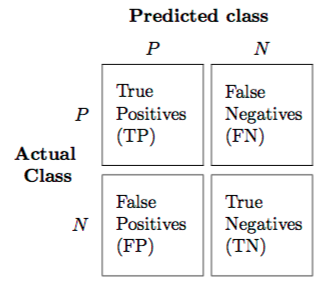
\includegraphics[scale=0.55]{Figures/confusion_matrix_1.png}
    \caption{Confusion Matrix}
    \label{fig:CM}
\end{figure}
\noindent
Above figure shows the confusion matrix. For our system,
\begin{itemize}
    \item True Positive(TP): Number of documents that is suspicious and also classified as suspicious.
    \item True Negative(TN): Number of documents that is non suspicious and also classified as non suspicious.
    \item False Negative(FN): Number of documents that is suspicious but classified as non suspicious.
    \item False Positive(FP): Number of documents that is non suspicious but classified as suspicious. 
\end{itemize}
\noindent
This numbers are used to calculate other evaluation measures.

\subparagraph{Precision :}
Precision referrers as positive predictive value. That is the ratio of
correctly classified positive instances to the total number of instances classified as positive. Precision can be obtained form  the following equation.
\begin{equation}
    \texttt{Precision} = \frac{TP}{TP+FP}
\end{equation}
If precision is high then the algorithm is doing well.

\subparagraph{Recall :}
Recall is the ratio of correctly classified positive instances to the total number of positive instances. It is also called true positive rate. Recall can be obtained from the following equation.
\begin{equation}
    \texttt{Recall} = \frac{TP}{TP+FN}
\end{equation}
High precision and high Recall is essential for a model. Unfortunately there is a trade-off between precision and recall. That is, improving precision typically reduces recall and vice versa. 
\begin{itemize}
    \item If threshold of a classifier is increased then it causes high precision and low recall.
    \item If threshold of a classifier is decreased then it causes low precision and high recall.
\end{itemize}
To sort out this problem we need another measure that is $F_1$measure.

\subparagraph{$F_1$ score :}
 $F_1$ score is the weighted average of Precision and Recall. Therefore, this score takes both false positives and false negatives into account. $F_1$ is usually more useful than accuracy. Accuracy works best if false positives and false negatives have similar cost. If the cost of false positives and false negatives are very different, it’s better to look at both Precision and Recall. F1-score can be obtained from the following equation,
 \begin{equation}
     F_1 = \frac{2*precision*recall}{precision+recall}
 \end{equation}
To chose a learning algorithm between several algorithms we have to find $F_1$ Score of algorithms. The algorithm which has highest $F_1$ score value is chosen as our learning algorithm.

\subparagraph{Accuracy :}
 Accuracy is the most intuitive performance measure and it is simply a ratio of correctly predicted observation to the total observations. For our system accuracy can be obtained by following equation,
\begin{equation}
    \texttt{Accuracy } = \frac{TP+TN}{TP+TN+FP+FN}
\end{equation}

Error of our system can be obtained easily after calculating accuracy,
\begin{equation}
    \texttt{Error} = 1-\texttt{Accuracy}
\end{equation}
We use two graphical measure to evaluate our system. These measures are,
\subparagraph{Precision Recall Curve :}
Precision Recall curves summarize the trade-off between the true positive rate and the positive predictive value for a predictive model using different probability thresholds. A precision-recall curve is a plot of the precision (y-axis) and the recall (x-axis) for different thresholds.

\subparagraph{ROC Curve :}
Receiver Operating Characteristic (ROC) Curves summarize the trade-off between the true positive rate and false positive rate for a predictive model using different probability thresholds. ROC curves are appropriate when the observations are balanced between each class. It is a plot of the false positive rate (x-axis) versus the true positive rate (y-axis) for a number of different candidate threshold values between 0 and 1.

\section{Experimental Results}
Table 5.3 represents Accuracy and Error rate of different classification algorithm on our dataset.
\renewcommand{\arraystretch}{1.5}
\begin{table}[h!]
\begin{center}
\caption{Evaluation Summary}
\begin{tabular}{|m{7cm} | m{3cm}| m{3cm}|}
\hline
     & Accuracy (\%) & Error (\%) \\
\hline
    Naive Bayes & 0.85 & 0.15\\
\hline 
    SVM (Linaer Kernel) & 0.91 & 0.09\\
\hline 
    SVM (RBF Kernel) & 0.90 & 0.10\\
\hline 
    Logistic Regression & 0.92 & 0.08\\
\hline
    K-Nearest Neighbor & 0.73 & 0.27\\
\hline
    Decision Tree & 0.88 & 0.12\\
\hline
\end{tabular}
\end{center}
\end{table}
\par
\noindent
From the evaluation summary we can see that Logistic Regression and Support Vector Machine algorithm's are performing up to the mark on our dataset . Naive Bayes and Decision tree also doing really well. But accuracy of K-nearest neighbour is really poor compare to other algorithms. 
\clearpage
\noindent
Table 5.4 shows the precision, recall and $F_1$ score of different classification algorithm used in our model.

\begin{table}[h!]
\begin{center}
\caption{Comparison of Results}
\begin{tabular}{|m{6.8cm} | m{2cm}| m{2cm}| m{2cm}|}
\hline
     & Precision & Recall & $F_1$ score \\
\hline
    Naive Bayes & 0.89 & 0.85 & 0.85\\
\hline 
    SVM (Linaer Kernel) & 0.91 & 0.91 & 0.91\\
\hline 
    SVM (RBF Kernel) & 0.90 & 0.91 & 0.90\\
\hline 
    Logistic Regression & 0.91 & 0.93 & 0.93\\
\hline
    K-Nearest Neighbor & 0.82 & 0.73 & 0.70\\
\hline
    Decision Tree & 0.88 & 0.92 & 0.89\\
\hline
\end{tabular}
\end{center}
\end{table}
\noindent
For all of the algorithms we use similar number of test documents. Logistic Regression performs well than other algorithm.
\par
\vspace{0.5cm}
\noindent
Table 5.4 shows comparison among six algorithms algorithms that were used in our system successfully. The $F_1$ score of Naive Bayes algorithm is 0.85 which is quite well. The result of SVM with linear kernel is quite similar as SVM with RBF kernel. But Linear kernel has better $F_1$ score than RBF kernel. Logistic Regression outperform all other algorithm, it has $F_1$ score of 0.93. Decision tree also performs well but $F_1$ score of K-nearest neighbor is the lowest.

\par
\vspace{0.5cm}
\noindent
Now, we will learn about classification report, Precision Recall curve and Receiver operating characteristic's (ROC) curve of  all of this algorithms. Classification report gives us precision, recall and $F_1$ score of each category which is really helpful to analyze the algorithm. From classification report we can see what category our model can can more accurately and what should we do to increase the accuracy of the system. Precision Recall curve and ROC curve shows the graphical evaluation of algorithms. Precision Recall curve shows value of precision and recall at different threshold values. ROC curve shows relation between true positive rate and false positive rate. 
\clearpage

%%%%%%%%% Naive Bayes Classifier %%%%%%%%%%%
%%%%%%%%%%%%%%%%%%%%%%%%%%%%%%%%%%%%%%
\subsection{Result of Naive Bayes Classifier}
Table 5.5 shows the classification report for Naive Bayes classifier. Here support expose the total number of document test by the system.

\begin{table}[h!]
\begin{center}
\caption{Classification Report (Naive Bayes)}
\begin{tabular}{|m{4.4cm} | m{2cm}| m{2cm}| m{2cm}| m{2cm}|}
\hline
     & Precision & Recall & $F_1$ score & Support \\
\hline
     Suspicious & 1.00 & 0.71 & 0.83 & 89\\
\hline 
     Non suspicious  & 0.76 & 1.00 & 0.87 & 84\\
\hline 
     avg./total & 0.89 & 0.85 & 0.85 & 173\\
\hline
\end{tabular}
\end{center}
\end{table}

\noindent
\textbf{Fig.} \ref{fig:prn} shows precision recall curve for Naive Bayes classifier.

\begin{figure}[h!]
    \centering
    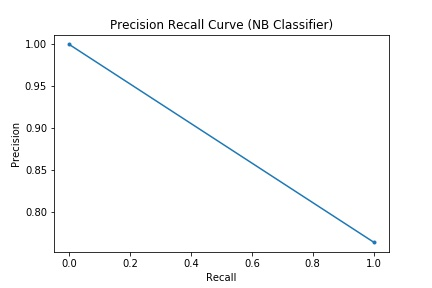
\includegraphics[scale=0.58]{Figures/PRN.jpg}
    \caption{Precision Recall Curve (Naive Bayes)}
    \label{fig:prn}
\end{figure}

\noindent
\textbf{Fig.} \ref{fig:rocn} shows ROC curve for Naive Bayes classifier.

\begin{figure}[h!]
    \centering
    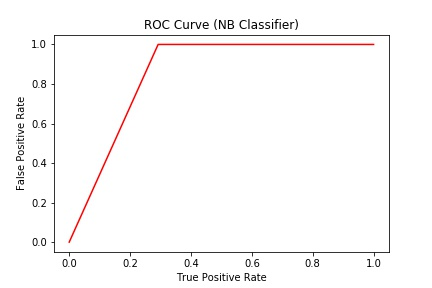
\includegraphics[scale=0.58]{Figures/ROCN.jpg}
    \caption{ROC Curve (Naive Bayes)}
    \label{fig:rocn}
\end{figure}

%%%%%%%%% SVM Linear kernel%%%%%%%%%%%
%%%%%%%%%%%%%%%%%%%%%%%%%%%%%%%%%%%%%%

\subsection{Result of SVM (Linear Kernel)}
Table 5.6 shows the classification report for Support Vector Machine with linear kernel.

\begin{table}[h!]
\begin{center}
\caption{Classification Report (SVM Linear Kernel)}
\begin{tabular}{|m{4.4cm} | m{2cm}| m{2cm}| m{2cm}| m{2cm}|}
\hline
     & Precision & Recall & $F_1$ score & Support \\
\hline
     Suspicious & 0.91 & 1.00 & 0.91 & 89\\
\hline 
     Non suspicious  & 1.00 & 0.90 & 0.91 & 84\\
\hline 
     avg./total & 0.91 & 0.91 & 0.91 & 173\\
\hline
\end{tabular}
\end{center}
\end{table}

\noindent
\textbf{Fig.} \ref{fig:prsl} shows precision recall curve for SVM (Linear Kernel).

\begin{figure}[h!]
    \centering
    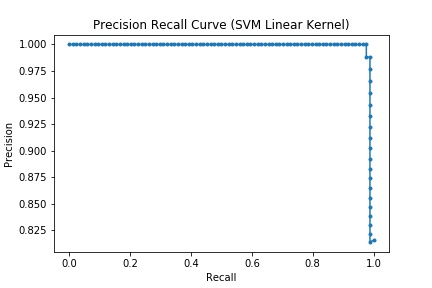
\includegraphics[scale=0.58]{Figures/PRSL.jpg}
    \caption{Precision Recall Curve (SVM Liner Kernel)}
    \label{fig:prsl}
\end{figure}

\noindent
\textbf{Fig.} \ref{fig:rocsl} shows ROC curve for SVM (Linear Kernel).

\begin{figure}[h!]
    \centering
    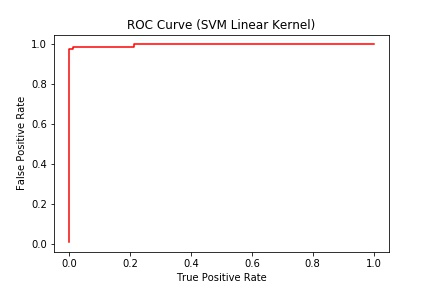
\includegraphics[scale=0.58]{Figures/ROCSL.jpg}
    \caption{ROC Curve (SVM Linear Kernel)}
    \label{fig:rocsl}
\end{figure}

%%%%%%%%% SVM RBF kernel%%%%%%%%%%%
%%%%%%%%%%%%%%%%%%%%%%%%%%%%%%%%%%

\subsection{Result of SVM (RBF Kernel)}
Table 5.7 shows the classification report for Support Vector Machine with RBF or Gaussian kernel.

\begin{table}[h!]
\begin{center}
\caption{Classification Report (SVM RBF Kernel)}
\begin{tabular}{|m{4.4cm} | m{2cm}| m{2cm}| m{2cm}| m{2cm}|}
\hline
     & Precision & Recall & $F_1$ score & Support \\
\hline
     Suspicious & 0.90 & 0.99 & 0.90 & 89\\
\hline 
     Non suspicious  & 0.99 & 0.89 & 0.91 & 84\\
\hline 
     avg./total & 0.90 & 0.91 & 0.90 & 173\\
\hline
\end{tabular}
\end{center}
\end{table}

\noindent
\textbf{Fig.} \ref{fig:prsk} shows precision recall curve for SVM (RBF Kernel).

\begin{figure}[h!]
    \centering
    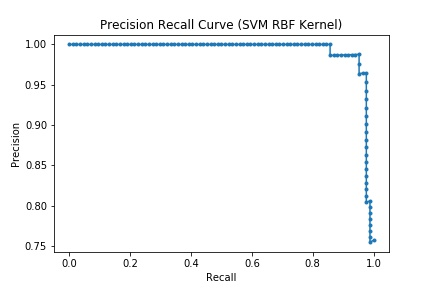
\includegraphics[scale=0.58]{Figures/PRSK.jpg}
    \caption{Precision Recall Curve (SVM RBF Kernel)}
    \label{fig:prsk}
\end{figure}

\noindent
\textbf{Fig.} \ref{fig:rocsk} shows ROC curve for SVM (RBF Kernel).

\begin{figure}[h!]
    \centering
    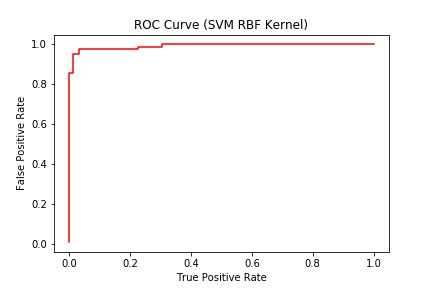
\includegraphics[scale=0.58]{Figures/ROCSK.jpg}
    \caption{ROC Curve (SVM RBF Kernel)}
    \label{fig:rocsk}
\end{figure}

%%%%%%% Logistic Regression %%%%%%%
%%%%%%%%%%%%%%%%%%%%%%%%%%%%%%%%%%%

\subsection{Result of Logistic Regression}
Table 5.8 shows the classification report for Logistic Regression.

\begin{table}[h!]
\begin{center}
\caption{Classification Report (Logistic Regression)}
\begin{tabular}{|m{4.4cm} | m{2cm}| m{2cm}| m{2cm}| m{2cm}|}
\hline
     & Precision & Recall & $F_1$ score & Support \\
\hline
     Suspicious & 0.92 & 1.00 & 0.93 & 89\\
\hline 
     Non suspicious  & 1.00 & 0.93 & 0.93 & 84\\
\hline 
     avg./total & 0.91 & 0.93 & 0.93 & 173\\
\hline
\end{tabular}
\end{center}
\end{table}

\noindent
\textbf{Fig.} \ref{fig:prl} shows precision recall curve for Logistic Regression.

\begin{figure}[h!]
    \centering
    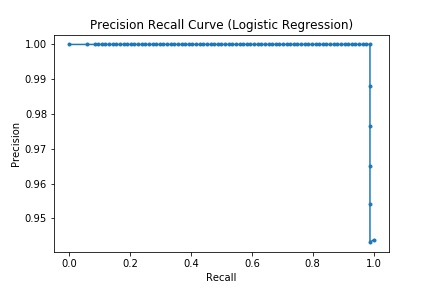
\includegraphics[scale=0.58]{Figures/PRL.jpg}
    \caption{Precision Recall Curve (Logistic Regression)}
    \label{fig:prl}
\end{figure}

\noindent
\textbf{Fig.} \ref{fig:rocl} shows ROC curve for Logistic Regression.

\begin{figure}[h!]
    \centering
    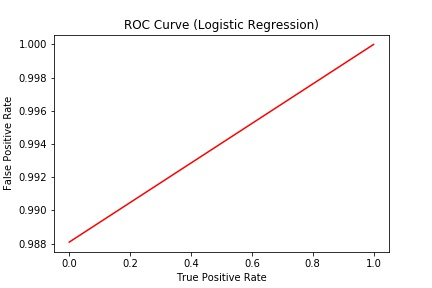
\includegraphics[scale=0.58]{Figures/ROCL.jpg}
    \caption{ROC Curve (Logistic Regression)}
    \label{fig:rocl}
\end{figure}

%%%%%%%% K-Nearest Neighbor %%%%%
%%%%%%%%%%%%%%%%%%%%%%%%%%%%%%%%%

\subsection{Result of K-Nearest Neighbor}
Table 5.9 shows the classification report for K-Nearest Neighbor.

\begin{table}[h!]
\begin{center}
\caption{Classification Report (K-Nearest Neighbor)}
\begin{tabular}{|m{4.4cm} | m{2cm}| m{2cm}| m{2cm}| m{2cm}|}
\hline
     & Precision & Recall & $F_1$ score & Support \\
\hline
     Suspicious & 0.65 & 1.00 & 0.79 & 89\\
\hline 
     Non suspicious  & 1.00 & 0.44 & 0.61 & 84\\
\hline 
     avg./total & 0.82 & 0.73 & 0.70 & 173\\
\hline
\end{tabular}
\end{center}
\end{table}

\noindent
\textbf{Fig.} \ref{fig:prknn} shows precision recall curve for K-Nearest Neighbor.

\begin{figure}[h!]
    \centering
    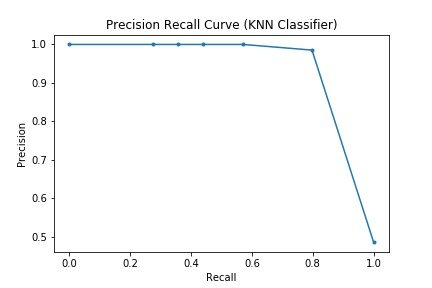
\includegraphics[scale=0.58]{Figures/PRKNN.jpg}
    \caption{Precision Recall Curve (K-Nearest Neighbor)}
    \label{fig:prknn}
\end{figure}

\noindent
\textbf{Fig.} \ref{fig:rocknn} shows ROC curve for K-Nearest Neighbor.

\begin{figure}[h!]
    \centering
    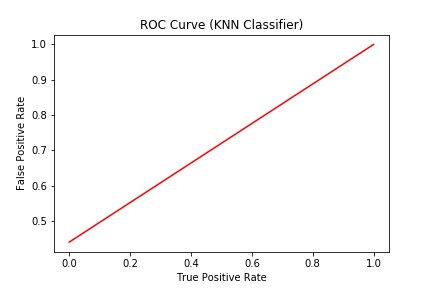
\includegraphics[scale=0.58]{Figures/ROCKNN.jpg}
    \caption{ROC Curve (K-Nearest Neighbor)}
    \label{fig:rocknn}
\end{figure}

%%%%%%%%%%%% Decision Tree %%%%%%%%%%%%
%%%%%%%%%%%%%%%%%%%%%%%%%%%%%%%%%%%%%%%
\subsection{Result of Decision Tree}
Table 5.10 shows the classification report for Decision Tree.

\begin{table}[h!]
\begin{center}
\caption{Classification Report (Decision Tree)}
\begin{tabular}{|m{4.4cm} | m{2cm}| m{2cm}| m{2cm}| m{2cm}|}
\hline
     & Precision & Recall & $F_1$ score & Support \\
\hline
     Suspicious & 0.91 & 0.89 & 0.90 & 89\\
\hline 
     Non suspicious  & 0.88 & 0.90 & 0.89 & 84\\
\hline 
     avg./total & 0.90 & 0.90 & 0.90 & 173\\
\hline
\end{tabular}
\end{center}
\end{table}

\noindent
\textbf{Fig.} \ref{fig:prdct} shows precision recall curve for Decision Tree.

\begin{figure}[h!]
    \centering
    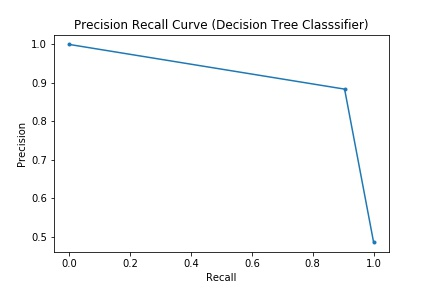
\includegraphics[scale=0.58]{Figures/PRDCT.jpg}
    \caption{Precision Recall Curve (Decision Tree)}
    \label{fig:prdct}
\end{figure}

\noindent
\textbf{Fig.} \ref{fig:rocdct} shows ROC curve for Decision Tree.

\begin{figure}[h!]
    \centering
    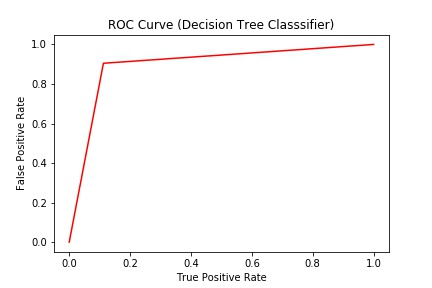
\includegraphics[scale=0.58]{Figures/ROCDCT.jpg}
    \caption{ROC Curve (Decision Tree)}
    \label{fig:rocdct}
\end{figure}

\section{Discussion}

After analyzing experimental results of all six algorithms we can conclude that Logistic Regression is the best learning algorithm for our system to detect/classify suspicious Bangla text. As discussed earlier Logistic Regression is a preferable model for binary classification. As ours is a binary classification problem, Logistic Regression is well suited for  our system. Performance of SVM is also good. In fact, this two algorithm shows quite similar results. We can also use it in our system as it is a very powerful machine learning algorithm.
\par 
\vspace{0.5cm}
\noindent
The performance of Naive Bayes algorithm and Decision Tree algorithm is also quite well. Increase in the number of training documents may increase efficiency of this algorithms. Among the algorithms the performance of K-Nearest Neighbor is the lowest. By changing the cluster size the efficiency of this algorithm can be increased.
\par 
\vspace{0.5cm}
\noindent
The overall accuracy of all algorithm can be increased by removing more stop words form our training examples. This words has no contribution in classifying the text. Occurrence of these words biases our algorithms which cause decrease in algorithm efficiency.  